\usetikzlibrary{arrows.meta}
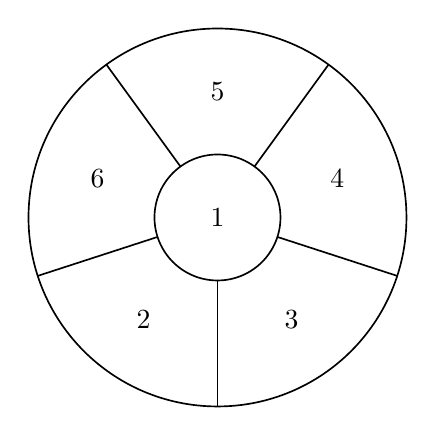
\begin{tikzpicture}[x=1cm,y=1cm,line width=0.6pt,font=\normalsize]
\coordinate (O) at (0,0);
\draw (O) circle[radius=2.4cm];
\draw (O) circle[radius=0.8cm];
\draw (54:0.8cm) -- (54:2.4cm);
\draw (126:0.8cm) -- (126:2.4cm);
\draw (198:0.8cm) -- (198:2.4cm);
\draw (270:0.8cm) -- (270:2.4cm);
\draw (342:0.8cm) -- (342:2.4cm);
\node[inner sep=0pt] at (O) {$1$};
\node[inner sep=0pt] at (90:1.6cm) {$5$};
\node[inner sep=0pt] at (18:1.6cm) {$4$};
\node[inner sep=0pt] at (306:1.6cm) {$3$};
\node[inner sep=0pt] at (234:1.6cm) {$2$};
\node[inner sep=0pt] at (162:1.6cm) {$6$};
\end{tikzpicture}
